% !TEX root = main.tex

\section{EyeNav}

\begin{figure}[h]
	\centering
	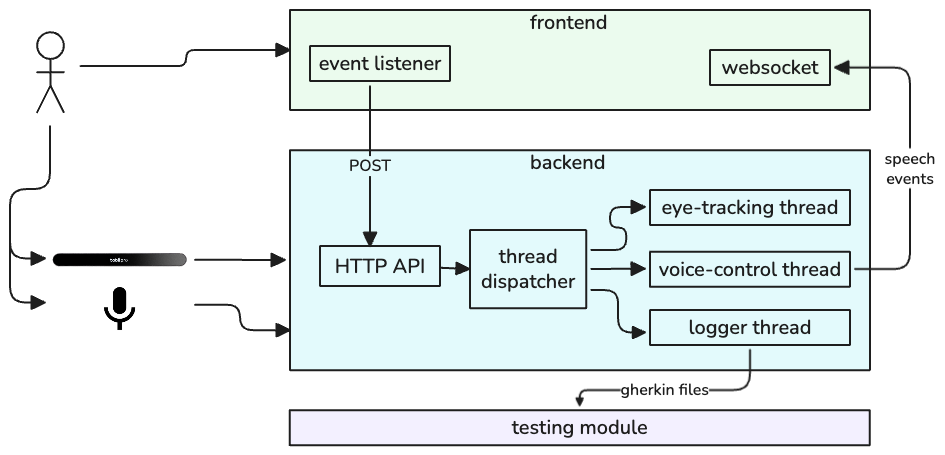
\includegraphics[width=220pt]{imgs/diagram-context.png}
	\caption{Context diagram of the system.}
	% \vspace{-13pt}
	\label{fig:context}
\end{figure}

This section outlines the EyeNav system based on its workflow, as illustrated in Fig.~\ref{fig:context}. EyeNav is composed of 2 main modules: (i) a Chrome Extension sidebar and (ii) a backend module built in python. The Chrome extension sidebar, which functions as an adjacent webpage alongside the main content, presents the available verbal commands, allows to initiate a interaction session, and shows the interpreted verbal commans in realtime once a session has started (See Fig.~\ref{fig:requirements}). Once a session begins, the system orchestrates multiple components, including voice recognition, eye tracking, and interaction logging.

\begin{figure}[h]
	\centering
	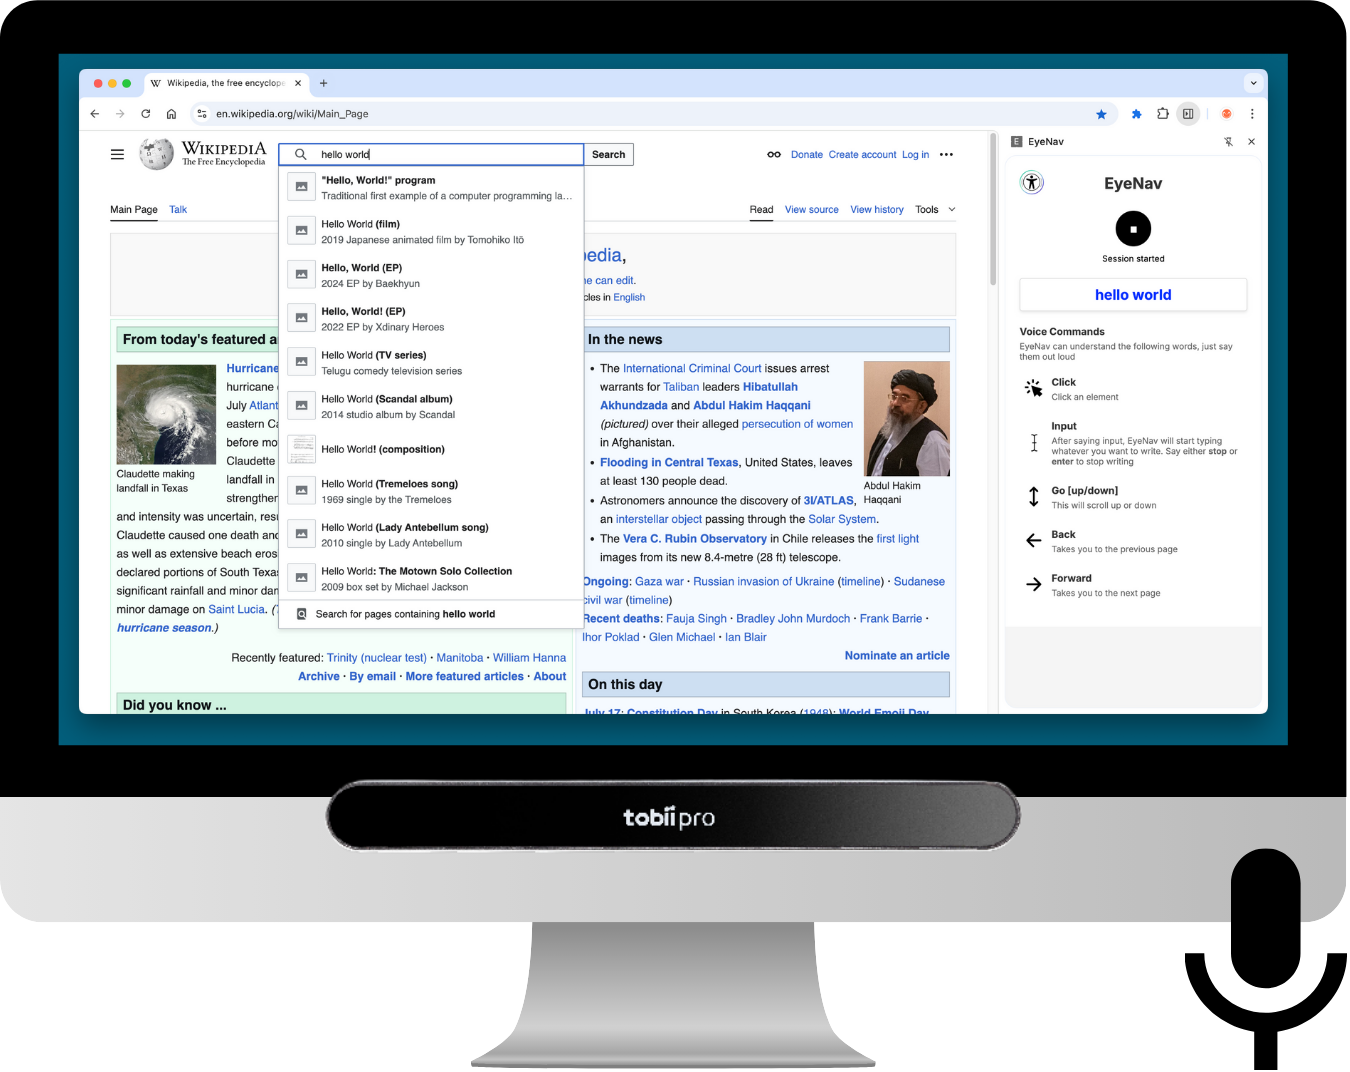
\includegraphics[width=210pt]{imgs/system-requirements.png}
	\caption{A graphic of what the system looks like}
	% \vspace{-13pt}
	\label{fig:requirements}
\end{figure}

User input is captured via an eye tracker and microphone, while the underlying processing occurs in a backend service rather than on the frontend. Concurrently, user interactions, such as clicks, text input, and navigation events, are recorded by a logging module. These recorded events are compiled into an executable test file, which can later be replayed using Gherkin-based test execution tools like Selenium\misref or Kraken\misref.

%\begin{figure}
%    \centering
%    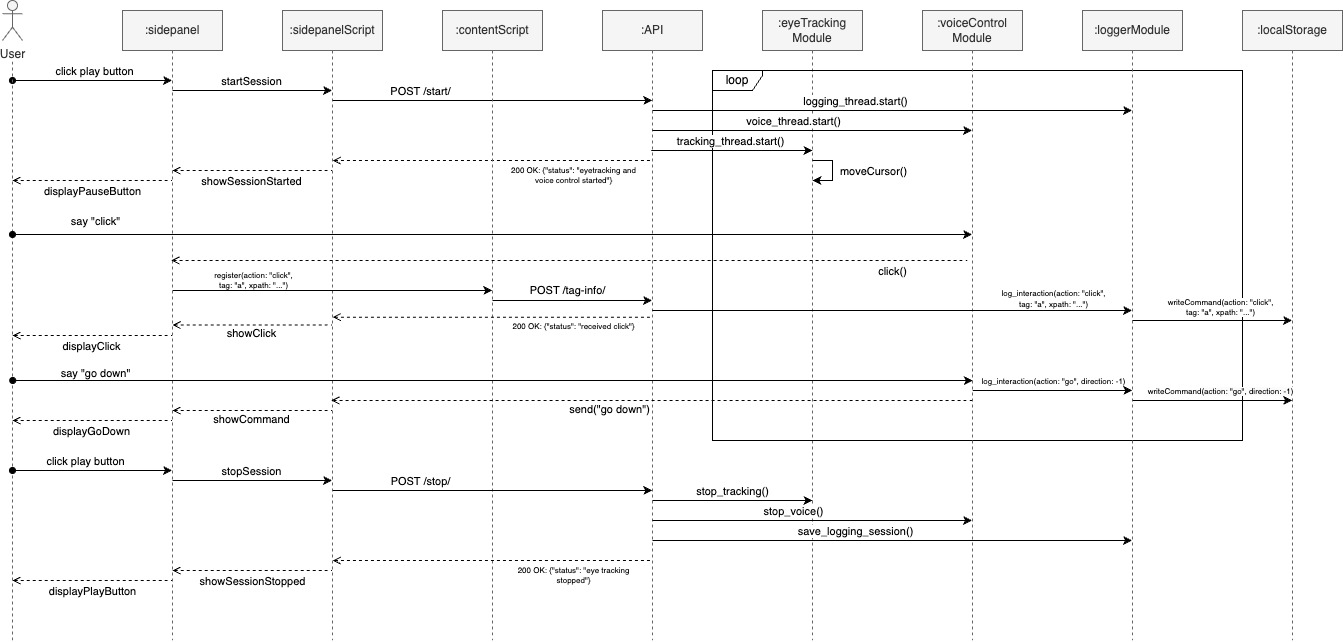
\includegraphics[width=210pt]{imgs/sequence-diagram.jpg}
%    \caption{Sequence diagram. The user starts a session, clicks, scrolls down and then stops the session.}
%    % \vspace{-13pt}
%    \label{fig:sequence-diagram}
%\end{figure}




\subsection{High-Level Architecture}

\begin{figure}
    \centering
    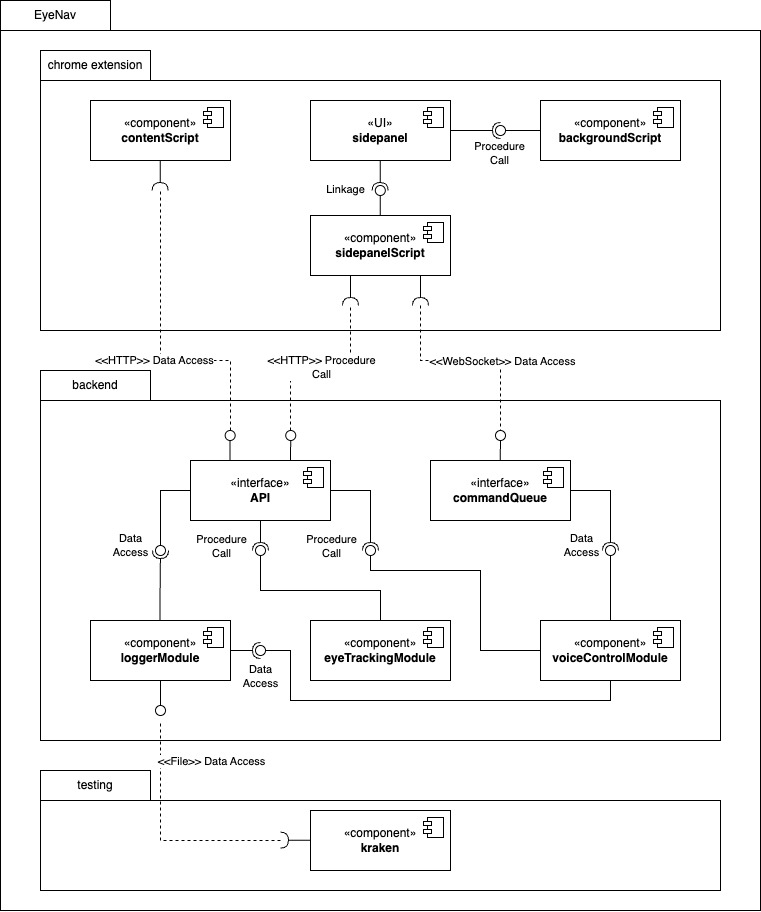
\includegraphics[width=210pt]{imgs/components-diagram.jpg}
    \caption{Components diagram}
    % \vspace{-13pt}
    \label{fig:components-diagram}
\end{figure}

% TODO poner todas las citas de las herramientas

Figure ~\ref{fig:components-diagram} presents the complete component architecture of the system.%, while Figure ~\ref{fig:sequence-diagram} illustrates the system in operation.

The Chrome extension serves as the front-end interface, providing real-time textual feedback for recognized voice commands and capturing user interaction events. Click events are recorded on the frontend and forwarded as HTTP POST requests to the backend to preserve contextual information, such as the associated HTML tag. 

Eye tracking is powered by the Tobii Pro Nano, a single-camera dark/bright pupil system with corneal reflection and a typical latency of approximately 17 ms~\cite{tobiiabndpronano}. The gaze-driven pointer control module uses the \verb|tobii-research| Python SDK to access real-time gaze data and interpolate cursor movement accordingly.

Voice commands are captured through a microphone and transcribed using the Vosk speech recognition engine\misref, which operates entirely on-device for privacy and low latency. Recognized phrases are matched to predefined command templates and sent to the backend over WebSocket connections, enabling minimal response delay.

The backend integrates data from both the Tobii eye tracker and the Vosk engine to interpret user intent, translate inputs into executable UI commands (e.g., clicks, scrolls, text entry), and log all interactions. A dedicated test logging module records each event in Gherkin syntax and compiles reproducible test scripts. These are executed using Kraken, a behavior-driven testing framework built on WebdriverIO\misref, supporting usability and regression testing even under dynamic UI conditions.

The system is organized into modular components, each adhering to a single-responsibility design principle. These include: (1) the gaze-driven pointer control, which enables real-time cursor positioning based on eye movement; (2) the NLP-based command parsing module, which interprets speech input captured by Vosk and maps it to specific UI actions among clicks, text entry, and scrolling; and (3) the record-and-replay test generation module, which logs user interactions in Gherkin syntax and compiles them into executable test scripts compatible with WebdriverIO for automated testing.

\section{EyeNav Capabilities}

\subsection{Voice Commands}

explain briefly the possible commands and how they are interpreted to ensure they are applied (for example, the different ways an element can be identified (id, xpath, ...))

\subsection{NLP in multiple languages}

\subsection{Test Case generation}

Add and example of a generated feature

\subsection{Accessible Interaction (Tab-based and voice-over)}

\section{EyeNev Use Cases}

\CAMILO{Mention the usage case details and the modules that could be "enable" to improve the results, for example for disable users the system does not require test case generation}

\subsection{Accesible Interaction mechanism for web applications}

\subsection{Record and Replay Testing Tool (A-TDD)}

\subsection{Accessibility Experts}

\subsection{Intelligent Agents}

%\section{EyeNav in action}
%
%% \begin{figure}
%%     \centering
%%     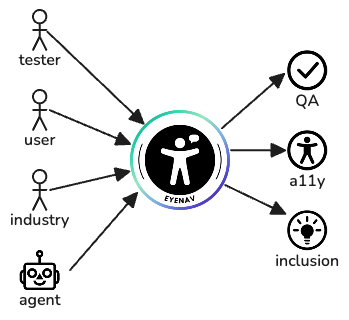
\includegraphics[width=160pt]{imgs/diagram-benefits.png}
%%     \caption{Envisioned users and the possible benefits from using the system}
%%     % \vspace{-13pt}
%%     \label{fig:benefits}
%% \end{figure}
%
%A typical use case starts with the user opening a browser window and launching the Chrome extension side panel. Prior to initialization, the eye tracker is calibrated, and the backend server starts running. When the user hits the start button, the servers starts listening for gaze and voice input, while recording each action in the testing module.
%
%For example: The user gazes at a search bar. $\rightarrow$ Says: “Click.” $\rightarrow$ Says: “Input Nike black shoes.” $\rightarrow$ Says: “Scroll down.” $\rightarrow$ Gazes at a product listing.$\rightarrow$ Says: “Click.”
%
%The recognized commands appear in a side panel for transparency, while the corresponding event interactions are logged by the backend testing module. These logs are stored locally as Gherkin features and step definitions, forming executable test files.


\section{Results}

\subsection{User Feedback}

Qualitative interviews identified several key usability factors. Larger UI elements significantly improved gaze accuracy, making it easier for users to select targets with their eyes. Voice commands were most effective when they were short and distinct, reducing recognition errors. Environmental noise was found to negatively impact the reliability of speech recognition, suggesting the need for robust filtering or alternative input strategies. Users also indicated that visual indicators for "gaze hover targets" would enhance feedback and confidence during interaction. Additionally, simplified scroll commands were perceived as more usable and intuitive compared to earlier, more granular versions.

\subsection{Accessibility Insights}

Testers noted that this input method offers clear benefits for users with limited motor function. However, improvements in UI design (e.g., reachable icons) are needed for full accessibility compliance. Due to scope limitations, no participants with motor impairments were included, though future studies aim to address this.

% the design of planned studies (for early prototypes)

\section{Discussion}

The integration of eye-tracking and NLP proved effective for hands-free interaction in a browser context. Further work is needed to improve performance in varied environments (e.g., low-light, users with glasses, non-native accents). Eye-based clicking was responsive but may require calibration for precision.

The testing module provided reproducible, human-readable test cases for interaction flows. While brittle on dynamic pages, these cases proved valuable for visual regression or task analysis. 

This architecture design allows for the combination of many of the purposes eye-tracking has already; we can analyze user behavior, identify usability bottlenecks, and validate system performance under varying conditions. This is especially valuable in eye-tracking based systems, where subtle differences in gaze patterns can significantly influence interaction outcomes. Replay tools also facilitate comparative evaluations, allowing different interface versions or input modalities to be tested using identical interaction sessions.

% \subsection{Planned Studies}
% TODO

\section{Future Work}

Planned improvements include enhancing support for users who wear glasses through prescription lens calibration techniques, and extending system compatibility to mobile and AR/VR platforms. Additional enhancements involve creating onboarding guides and integrating visual cues to facilitate learning gaze-based input, as well as including individuals with motor impairments in future user studies to better validate accessibility benefits. The system's test recorder is also being developed as a standalone tool to support broader usability testing efforts. Finally, there are plans to explore integration with immersive environments, such as the Apple Vision Pro and Meta Quest, to evaluate usability and responsiveness in mixed-reality contexts.
